
\section{Warkocze}
\label{sec:braid}%
\index{warkocz|(}%
Warkocze, a dokładniej grupa warkoczy, rozważane po raz pierwszy były niejawnie przez Hurwitza w~pracy z~1891 roku o~monodromii oraz jawnie przez Artina \cite{artin25} w~1925 roku.
\index[persons]{Artin, Emil}%
Dla nas głównym źródłem wiedzy była wspaniała praca przeglądowa Birman, Brendle \cite{birman05} poświęcona warkoczom, ale też notatki Gonzáleza-Menesesa \cite{gonzalez11} z~kursu zorganizowanego w~Pau.
\index[persons]{Birman, Joan}%
\index[persons]{Brendle, Tara}%
\index[persons]{González-Meneses, Juan}%

Żałujemy, że nie odkryliśmy wcześniej przyjemnej w lekturze i pięknie ilustrowanej książki Kassela, Turajewa \cite{kassel08}, którą polecamy każdemu, kto chce poświęcić się teorii warkoczy.
\index[persons]{Kassel, Christian}%
\index[persons]{Turajew, Władymir (Тураев, Владимир Георгиевич)}%
Ta ostatnia pozycja obejmuje wszystko, o czym piszemy my, a dodatkowo też reprezentację Lawrence'a-Krammera-Bigelowa, makaron i widelce, algebry Iwahoriego-Heckego albo ślady Ocneanu oraz wiele innych tematów.
\index{reprezentacja!Lawrence'a-Krammera-Bigelowa}%
\index{makaron i widelce}%
\index{algebra!Iwahoriego-Heckego}%
\index{ślad Ocneanu}%

% DICTIONARY;braid;warkocz;-
% DICTIONARY;strand;pasmo ...;warkocz
\begin{definition}[warkocz]
\index{pasmo warkocza}%
O dwóch punktach $(d_1, t_1)$, $(d_2, t_2)$ w~walcu $B^2 \times [0, 1] \subseteq \R^3$ powiemy, że łączący je odcinek jest malejący, jeśli $t_1 > t_2$.
Łamana malejąca to taka, która jest złożona z~odcinków malejących.
Teoriomnogościową sumę parami rozłącznych łamanych malejących, które łączą zbiory $\{x_1, \ldots, x_n\} \times \{1\}$ oraz $\{x_1, \ldots, x_n\} \times \{0\}$, nazywamy warkoczem o~$n$ pasmach.
\end{definition}

Poszczególne pasma warkocza możemy utożsamiać z~wykresami pewnych (gładkich) funkcji $f_i \colon [0, 1] \to \R^2$, jeśli zbiory $\{f_i(0) : 1 \le i \le n\} = \{f_i(1) : 1 \le i \le n\}$ są równe.
Intuicyjnie, wartości $f_i(0)$ opisują początki, a $f_i(1)$ końce pasm.

Wtedy dwa warkocze $f_1, f_2, \ldots, f_n$ oraz $g_1, g_2, \ldots, g_n$ uznajemy za równoważne, jeśli istnieje między nimi izotopia: funkcje ciągłe dwóch zmiennych $F_i(t, s)$ określone na zbiorze $[0,1] \times [0,1]$ takie, że $F_i(t,0)= f_i(t)$ oraz $F_i(t, 1) = g_i(t)$.
Przez analogię do węzłów można zdefiniować diagramy warkoczy jako cienie bez katastrof.
Najczęściej rzutujemy prostopadle do odcinka $\{0\} \times [0, 1]$.

\begin{definition}
\index{grupa warkoczy}%
    Określmy pomocniczo dwie kontrakcje $B^2 \times [0,1] \to B^2 \times [0,1]$:
    \begin{align*}
        \psi_1(d, t)&  = (d, t/2) \\
        \psi_2(d, t)&  = (d, \frac12 (t+1))
    \end{align*}
    Klasy abstrakcji warkoczy z~mnożeniem danym wzorem $z_1z_2 = \psi_1(z_1) \cup \psi_2(z_2)$ tworzą grupę warkoczy $B_n$.
    Jej elementem neutralnym jest warkocz $1_n = \bigcup_{i = 1}^n \{x_1\} \times [0,1]$.
\end{definition}

Sprawdzenie aksjomatów grupy pozostawiamy Czytelnikowi,
pozostawiając mu małą wskazówkę graficzną:
\begin{comment}
\[
    \begin{tikzpicture}[baseline=-0.65ex, scale=0.2]
    \begin{knot}[clip width=5, end tolerance=1pt]
        \strand[semithick] (-6, 0) .. controls (-4, 0) and (-5, 2) .. (-3, 2);
        \strand[semithick] (-6, 2) .. controls (-4, 2) and (-5, 0) .. (-3, 0);
        \strand[semithick] (-6, -2) to (-3, -2);
        \strand[semithick] (-3, 0) .. controls (-1, 0) and (-2, -2) .. (0, -2);
        \strand[semithick] (-3, -2) .. controls (-1, -2) and (-2, 0) .. (0, 0);
        \strand[semithick] (-3, 2) to (0, 2);
        \strand[semithick] (+6, 0) .. controls (+4, 0) and (+5, 2) .. (+3, 2);
        \strand[semithick] (+6, 2) .. controls (+4, 2) and (+5, 0) .. (+3, 0);
        \strand[semithick] (+6, -2) to (+3, -2);
        \strand[semithick] (+3, 0) .. controls (+1, 0) and (+2, -2) .. (0, -2);
        \strand[semithick] (+3, -2) .. controls (+1, -2) and (+2, 0) .. (0, 0);
        \strand[semithick] (+3, 2) to (0, 2);
        \draw (+6, -3) rectangle (0, 3);
        \draw (-6, -3) rectangle (0, 3);
        \draw[semithick, decoration={brace,mirror,raise=3pt},decorate]  (-5.75, -3) -- node[below=6pt] {$\beta$} (-0.25, -3);
        \draw[semithick, decoration={brace,mirror,raise=3pt},decorate]  (0.25, -3) -- node[below=6pt] {$\beta^{-1}$} (5.75, -3);
    \end{knot}
    \end{tikzpicture}
    \cong
    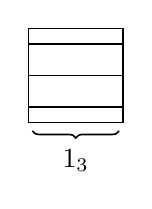
\begin{tikzpicture}[baseline=-0.65ex, scale=0.2]
        \draw[semithick] (-3, -2) to (3, -2);
        \draw[semithick] (-3, 0) to (3, 0);
        \draw[semithick] (-3, 2) to (3, 2);
        \draw (-3, -3) rectangle (3, 3);
        \draw[semithick, decoration={brace,mirror,raise=3pt},decorate]  (-2.75, -3) -- node[below=6pt] {$1_3$} (2.75, -3);
    \end{tikzpicture}
    \quad\quad\quad
    \begin{tikzpicture}[baseline=-0.65ex, scale=0.2]
        \useasboundingbox (-6, -3) rectangle (12, 5);
\begin{knot}[clip width=5, end tolerance=1pt]
        \strand[semithick] (-6, 0) .. controls (-4, 0) and (-5, 2) .. (-3, 2);
        \strand[semithick] (-6, 2) .. controls (-4, 2) and (-5, 0) .. (-3, 0);
        \strand[semithick] (-6, -2) to (-3, -2);
        \strand[semithick] (-3, 0) .. controls (-1, 0) and (-2, -2) .. (0, -2);
        \strand[semithick] (-3, -2) .. controls (-1, -2) and (-2, 0) .. (0, 0);
        \strand[semithick] (-3, 2) to (0, 2);
        \draw (-6, -3) rectangle (0, 3);
        \draw[semithick, decoration={brace,mirror,raise=3pt},decorate]  (-5.75, -3) -- node[below=6pt] {$\beta_1$} (-0.25, -3);
        \strand[semithick] (+6, 0) .. controls (+4, 0) and (+5, 2) .. (+3, 2);
        \strand[semithick] (+6, 2) .. controls (+4, 2) and (+5, 0) .. (+3, 0);
        \strand[semithick] (+6, -2) to (+3, -2);
        \strand[semithick] (+3, 0) .. controls (+1, 0) and (+2, -2) .. (0, -2);
        \strand[semithick] (+3, -2) .. controls (+1, -2) and (+2, 0) .. (0, 0);
        \strand[semithick] (+3, 2) to (0, 2);
        \draw (+6, -3) rectangle (0, 3);
        \strand[semithick] (6+6, 0) .. controls (6+4, 0) and (6+5, 2) .. (6+3, 2);
        \strand[semithick] (6+6, 2) .. controls (6+4, 2) and (6+5, 0) .. (6+3, 0);
        \strand[semithick] (6+6, -2) to (6+3, -2);
        \strand[semithick] (6+3, 0) .. controls (6+1, 0) and (6+2, -2) .. (6+0, -2);
        \strand[semithick] (6+3, -2) .. controls (6+1, -2) and (6+2, 0) .. (6+0, 0);
        \strand[semithick] (6+3, 2) to (6+0, 2);
        \draw (6+6, -3) rectangle (6+0, 3);
        \draw[semithick, decoration={brace,mirror,raise=3pt},decorate]  (0.25, -3) -- node[below=6pt] {$\beta_2\beta_3$} (11.75, -3);
        \draw[semithick, decoration={brace,raise=3pt},decorate]  (6.25, 3) -- node[above=6pt] {$\beta_3$} (11.75, 3);
        \draw[semithick, decoration={brace,raise=3pt},decorate]  (-5.75, 3) -- node[above=6pt] {$\beta_1\beta_2$} (5.75, 3);
    \end{knot}
    \end{tikzpicture}
\]
\end{comment}

\begin{proposition}
    Grupa warkoczy $B_n$ ma prezentację
    \begin{equation}
        \{\sigma_1, \ldots, \sigma_{n-1} : \sigma_i\sigma_{i+1} \sigma_i = \sigma_{i+1} \sigma_i \sigma_{i+1}, |i-j| \neq 1 \implies \sigma_i \sigma_j = \sigma_j \sigma_i\}.
    \end{equation}
\end{proposition}

Pierwszy był sam Artin \cite{artin25}, wiele lat później Birman, Ko, Lee odkryli nową, ,,symetryczną'' prezentację, ale dla oszczędności miejsca nawet ich nie cytujemy.
% MR1870512 albo MR1654165
\index[persons]{Artin, Emil}%
\index[persons]{Birman, Joan}%
\index[persons]{Ko, Ki}%
\index[persons]{Lee, Sang}%
Wraz z~upływem czasu pojawiły się nowe dowody (w~kolejności chronologicznej): Magnusa \cite{magnus34}, Bohnenblusta \cite{bohnenblust47}, Chow \cite{chow48}, Fadella i van Buskirka \cite{fadell62}, Foxa i Neuwirtha \cite{fox62}.
\index[persons]{Bohnenblus, Frederic}%
\index[persons]{Chow, Wei-Liang}%
\index[persons]{Fadell, Edward}%
\index[persons]{Fox, Ralph}%
\index[persons]{Magnus, Wilhelm}%
\index[persons]{Neuwirth, Lee}%
\index[persons]{van Buskirk, James}%
Patrz też do książki Birman \cite{birman74}.
González-Meneses \cite{gonzalez11} przytacza ze szczegółami niektóre dowody (przez czesanie warkoczy, grupy podstawowe kompleksów komórkowych i inne).

Generatory $\sigma_i$ posiadają nieskomplikowaną interpretację graficzną:
\begin{comment}
\[
    \begin{tikzpicture}[baseline=-0.65ex, scale=0.2]
    \begin{knot}[clip width=5, end tolerance=1pt]
        \strand[semithick] (-8, -4.5) to (8, -4.5);
        \strand[semithick] [in=left,out=right] (-8, -1.5) to (8, 1.5);
        \strand[semithick] [in=left,out=right] (-8, 1.5) to (8, -1.5);
        \strand[semithick] (-8, 4.5) to (8, 4.5);
        \node at (-10, -4.5) {$1$};
        \node at (-10, -3) {$\ldots$};
        \node at (-10, -1.5) {$i$};
        \node at (-10, 1.5) {$i+1$};
        \node at (-10, 3) {$\ldots$};
        \node at (-10, 4.5) {$n$};
        \node at (0, 3) {$\ldots$};
        \node at (0, -3) {$\ldots$};
    \end{knot}
    \end{tikzpicture}
\]
\end{comment}

Jeśli zapomnimy, jak poszczególne pasma krzyżują się, każdy warkocz staje się permutacją zbioru $n$-elementowego.
To odwzorowanie jest ,,na'' i zgodne ze składaniem warkoczy, dlatego wyznacza homomorfizm $B_n \to S_n$.
% DICTIONARY;pure;czysty;warkocz
\index{warkocz!czysty}%
Jego jądro stanowi podgrupa warkoczy czystych, czyli takich, że początek i~koniec każdego pasma znajdują się w~tej samej pozycji.

\begin{proposition}
    Grupa warkoczy $B_n$ jest przemienna wtedy i tylko wtedy, gdy $n = 1, 2$.
\end{proposition}

\begin{proof}
    Dla $n = 1$ grupa warkoczowa jest trywialna, dla $n = 2$ mamy $B_2 \cong \Z$.
    Załóżmy, że $n \ge 3$. Wtedy grupa symetrii $S_n$ jest nieprzemienna, zatem grupa $B_n$ także taka jest.
\end{proof}

Obrazem generatora $\sigma_i \in B_n$ jest transpozycja $(i, i+1) \in S_n$, co pozwala przepisać prezentację Artina grupy $B_n$ do prezentacji Coxetera grupy symetrii:
\index{prezentacja Coxetera grupy symetrii}%
\begin{equation}
    S_n = \langle s_1, \ldots, s_{n-1} \mid
    s_i^2 = 1,
    s_{i}s_{i+1}s_{i} = s_{i+1}s_{i}s_{i+1},
    s_is_j = s_js_i \mbox{ dla } |i-j| \neq 1 \rangle
\end{equation}

\begin{proposition}
    Jeśli $n \ge 3$, to centrum grupy $B_n$ jest generowane przez warkocz $(\prod_{i = 1}^{n-1} \sigma_i)^2$.
\end{proposition}

\begin{proof}[Niedowód]
\index[persons]{Garside, Frank}%
\index[persons]{Chow, Wei-Liang}%
    Zazwyczaj wskazuje się dowód Garside'a \cite{garside69}, ale pierwszy dowód opublikował Chow \cite{chow48}, o czym Garside pisze w abstrakcie swojej pracy.
\end{proof}

Grupa $B_3$ jest izomorficzna z grupą podstawową trójlistnika (patrz przykład~\ref{exm:trefoil_group}).
Nie istnieje żaden węzeł, którego grupą podstawową byłaby jednak $B_n$ dla $n \ge 4$: tam elementy $\sigma_1$, $\sigma_n$ oraz generator centrum rozpinają grupę izomorficzną z~$\Z^3$.
Natomiast asferyczna, niezwarta 3-rozmaitość nie może mieć grupy podstawowej $\Z^3$.
Musimy niestety pominąć czysto kohomologiczny dowód\footnote{Głodny wiedzy Czytelnik powinien odwiedzić \url{https://math.stackexchange.com/a/2119984}.} faktu, ale zaiste prowadzi to do sprzeczności.


\subsection{Warkocze a sploty}
% DICTIONARY;closure of ...;domknięcie ...;warkocz
Każdy warkocz można domknąć do węzła, łącząc ze sobą punkty $(x_i, 1)$ oraz $(x_i, 0)$ łamanymi, których rzuty do płaszczyzny diagramu nie przecinają się.
\index{warkocz!domknięcie warkocza}%
Nie wiadomo, kto wymyślił operację domykania warkoczy, ale była ona z pewnością znana Alexanderowi: rozpatrywano je jeszcze przed samymi warkoczami.
\index[persons]{Alexander, James}%
% TODO: rysunek w TikZ, jak się domyka.

\begin{theorem}[Alexander, 1923]
\index{twierdzenie!Alexandera}%
\label{thm:alexander}%
    Każdy splot powstaje przez domknięcie pewnego warkocza.
\end{theorem}

\begin{proof}[Niedowód]
    W kolejności chronologicznej:
    najpierw Alexander \cite{alexander23},
\index[persons]{Alexander, James}%
    a~po blisko połowie wieku Morton \cite{mortonhr86},
\index[persons]{Morton, Hugh}%
    Yamada \cite{yamada87} (co daje łatwy do zaimplementowania program komputerowy)
\index[persons]{Yamada, Shuji}%
    i~Vogel \cite{vogel90} (ulepszający algorym Yamady).
\index[persons]{Vogel, Pierre}%
\end{proof}

Manturow \cite{manturov02} pokazał, że od warkocza można wymagać kwazitoryczności (warkocz nazywamy torycznym, jeżeli jest postaci $(\sigma_1 \ldots \sigma_{p-1})^q$ oraz kwazitorycznym, jeżeli powstaje przez odwrócenie niektórych skrzyżowań z~warkocza torycznego).
\index[persons]{Manturow, Wasilij}%
\index{warkocz!toryczny}%
\index{warkocz!kwazitoryczny}%

\begin{theorem}[Markow, 1936]
\index{twierdzenie!Markowa}%
    Sploty powstałe przez domknięcie dwóch warkoczy są takie same wtedy i~tylko wtedy, gdy jeden warkocz powstaje z~drugiego przez ciąg sprzężeń: $z_1 \mapsto z_2 z_1 z_2^{-1}$ oraz procesów Markowa, które zastępują $n$-warkocz $\beta$ przez $(n+1)$-warkocz $\beta\sigma_n^{\pm 1}$.
\end{theorem}

\begin{proof}[Niedowód]
    Kompletny i~godny naśladowania dowód znajduje się w~trudno dostępnej książce Birman \cite{birman74}, więc warto sprawdzić inne, opublikowane później materiały:
\index[persons]{Birman, Joan}%
    Morton \cite{mortonhr86} opisał przepiękną, a~przy tym elementarną ideę ,,nitkowania'',
\index[persons]{Morton, Hugh}%
    potem Traczyk \cite{traczyk98} podał czysto kombinatoryczne, dwuwymiarowe uzasadnienie oparte o~okręgi Seiferta,
\index[persons]{Traczyk, Paweł}%
    wreszcie mamy też nowe geometryczne rozumowanie Birman, Menasco \cite{birman02} wykorzystujące foliacje.
\index[persons]{Menasco, William}%
\index{foliacja}%
\end{proof}

Pierwsze sformułowanie twierdzenia pochodzące od Markowa \cite{markov36} korzystało z~trzech ruchów, jeden z~nich stanowił uogólnienie II ruchu Reidemeistera.
\index[persons]{Markow, Andrej (Марков, Андрей Андреевич)}%
Weinberg \cite{weinberg39} zauważył trzy lata później, że wystarczą dwa ruchy.
\index[persons]{Weinberg, Noah}%
% Weinberg = Ной Вайнберг: http://www.mathsoc.spb.ru/history/Odynec_2020.pdf
Lambropoulou, Rourke \cite{lambropoulou97} przedstawili wersję twierdzenia wymagającą tylko jednego ,,L-ruchu''.
\index[persons]{Lambropoulou, Sofia}%
\index[persons]{Rourke, Colin}%

Historia twierdzenia Markowa jest raczej dramatyczna: Markow przedstawił swój dowód ustnie, ale nigdy go nie opublikował, zostawiając to zadanie swojemu uczniowi, Weinbergowi.
Ten jednak został zabity podczas wojny, wkrótce po opublikowaniu pierwszej pracy na temat teorii węzłów i~na dokładny dowód trzeba było czekać na Birman \cite{birman74} blisko 40 lat.
\index[persons]{Birman, Joan}%

Nie znamy wielu twierdzeń o warkoczach i splotach, jakie powstają przez ich domykanie.
Jones \cite{jones85} podał bez dowodu:

\begin{proposition}
    Niech $b \in B_n$ będzie słowem zapisanym na standardowych generatorach.
    Oznaczmy przez $b_+$, $b_-$ nieznakowaną sumę dodatnich, ujemnych wykładników.
    Jeśli $b_+ - 3b_- \ge n$, to domknięcie warkocza $b$ nie jest achiralne.
\index{węzeł!achiralny}%
\end{proposition}




\subsection{Reprezentacja Burau}
Na zakończenie sekcji wspomnijmy o~macierzowej reprezentacji Burau, wprowadzonej do matematyki w latach trzydziestych zeszłego wieku \cite{burau33}.
\index[persons]{Burau, Werner}%
\index{reprezentacja!Burau}%
Wyznaczona jest ona przez obrazy generatorów:
\begin{equation}
    \varphi(\sigma_i) = I_{i-1} \oplus \begin{pmatrix}
        1-t & t \\
        1   & 0
    \end{pmatrix} \oplus I_{n-i-1}
\end{equation}
Reprezentacja $\varphi$ jest wierna dla $n = 2, 3$, wiedziano o~tym od jakiegoś czasu. % wiedział to Magnus w 1969: https://mathscinet.ams.org/mathscinet-getitem?mr=264062
% dowód ma też Kassel, Turaev - strona 110
Moody \cite{moody91} pokazał, że reprezentacja nie jest wierna dla $n > 8$, Long, Paton \cite{paton93} ulepszyli jego podejście i~poprawili jego wynik do niewierności dla $n > 5$.
\index[persons]{Moody, John}%
\index[persons]{Paton, Mark}%
\index[persons]{Long, Darren}%
% Paton = Mark https://www.genealogy.math.ndsu.nodak.edu/id.php?id=139714
Ich kontrukcja korzysta z~pewnej zamkniętej krzywej na sześciokrotnie przekłutym dysku o~pewnych cechach homologicznych.
Podobnymi metodami Bigelow pokazał u schyłku stulecia \cite{bigelow99}, że jeśli
\index[persons]{Bigelow, Stephen}%
\begin{align}
    \psi_1 & = \sigma_3^{{-1}}\sigma_2\sigma_1^2\sigma_2\sigma_4^3\sigma_3\sigma_2, \\
\psi_2 & = \sigma_4^{{-1}}\sigma_3\sigma_2\sigma_1^{{-2}}\sigma_2\sigma_1^2\sigma_2^2\sigma_1\sigma_4^5,
\end{align}
to komutator $[\psi_1^{{-1}}\sigma_4\psi_1,\psi_2^{{-1}}\sigma_4\sigma_3\sigma_2\sigma_1^2\sigma_2\sigma_3\sigma_4\psi_2]$ należy do jądra.
Czy reprezentacja Burau dla $B_4$ jest wierna?
Negatywna odpowiedź na to pytanie prawie na pewno prowadziłaby do
nietrywialnego węzła, którego wielomianem HOMFLY jest $1$,
natomiast odpowiedź pozytywna raczej nie ma aż tak dramatycznych następstw.
% The first nonfaithful Burau representations were found by John A. Moody without the use of computer, using a notion of winding number or contour integration.[3] A more conceptual understanding, due to Darren D. Long and Mark Paton[4] interprets the linking or winding as coming from Poincaré duality in first homology relative to the basepoint of a covering space, and uses the intersection form (traditionally called Squier's Form as Craig Squier was the first to explore its properties).[5] Stephen Bigelow combined computer techniques and the Long–Paton theorem to show that the Burau representation is not faithful for n ≥ 5.[6][7][8] Bigelow moreover provides an explicit non-trivial element in the kernel as a word in the standard generators of the braid group: let




\subsection{Grupy warkoczy w algebrze}
Grupy $B_n$ mogą być obiektem badań algebry bez związku z~teorią węzłów.

\begin{proposition}
    Grupa warkoczy $B_n$ jest beztorsyjna dla każdego $n \ge 1$.
\end{proposition}

Istnieje wiele dowodów tego faktu: pierwszy korzystał z~krótkich ciągów dokładnych (Fadell, Neuwirth \cite{neuwirth1962}), później podano oparty o~struktury Garside'a (Garside \cite{garside1969}), czysto teoriogrupowy pochodzi od Dyera \cite{dyer1980}.
\index[persons]{Dyer, Joan}%
\index[persons]{Fadell, Edward}%
\index[persons]{Garside, Frank}%
\index[persons]{Neuwirth, Lee}%
My przedstawimy inne rozumowanie, opisując przy tym ciekawy sam w~sobie porządek Dehornoya\footnote{W 1989 roku udowodniono, że pewien aksjomat teorii mnogości, $I_3$, dotyczący dużych liczb kardynalnych implikuje istnienie algebraicznej struktury zwanej acykliczną półką (nie mylić z naszymi półkami).
To pociąga decydowalność problemu słowa dla prawa $x(yz) = (xy)(xz)$, coś co nie jest wprost związane z dużymi liczbami kardynalnymi.
Dehornoy w 1992 roku podał przykład acyklicznej półki na grupie warkoczy $B_\infty$.}.% z artykułu "Dehornoy order na wiki"
\index{porządek Dehornoya}%

\begin{proof}
\index[persons]{Dehornoy, Patrick}%
    Mówimy, że grupa $G$ jest lewo-porządkowalna, jeśli można wyposażyć ją w~zupełny porządek $<$, niezmienniczy na mnożenie z lewej strony.
    To znaczy, dla każdych $a, b, c \in G$, z~nierówności $a < b$ wynika $ca < cb$.
    Wtedy zbiór $P = \{g \in G \mid e < g\}$ nazywamy półgrupą elementów dodatnich.
    Łatwo widać, że $G$ jest sumą rozłączną $P \sqcup \{e\} \sqcup P^{-1}$.
    Odwrotnie, każde takie rozbicie wyznacza porządek: wystarczy zdefiniować $a < b \iff a^{-1}b \in P$.

    Dehornoy znalazł taki porządek dla grupy warkoczowej $B_n$ w~\cite{dehornoy1994}.
    Za zbiór $P$ elementów dodatnich wziął te słowa na standardowych generatorach, które dla pewnego $i$ zawierają $\sigma_i$, ale nie $\sigma_i^{-1}$ ani $\sigma_j^{\pm 1}$ dla $j < i$.
    Pokazanie, że $P$ jest półgrupą nie sprawia trudności, ale tego, że $B_n$ jest wtedy rozłączną sumą $P, P^{-1}$ i trywialnego warkocza stanowi co najmniej nietrywialne zadanie.

    Lewo-porządkowalna grupa jest beztorsyjna.
    Istotnie, ustalmy element $g \in G$ różny od elementu neutralnego.
    Bez straty ogólności niech $e < g$, przemnóżmy tę nierówność stronami przez $g$.
    Dostaniemy tak nową nierówność $g < g^2$.
    Powtarzając proces otrzymujemy łańcuch $e < g < g^2 < g^3 < \ldots$.
    Skoro $<$ jest porządkiem, nie jest możliwe by któryś z elementów $g^n$ był neutralny.
\end{proof}

Dowód uproszczono: Fenn, Greene, Rolfsen, Rourke i Wiest \cite{fenn1999} podali cztery lata później bezpośrednie geometryczne rozumowanie, które prowadzi do takiego samego porządku jak ten z pracy Dehornoya.
\index[persons]{Fenn, Roger}%
\index[persons]{Greene, Joshua}%
\index[persons]{Rolfsen, Dale}%
\index[persons]{Rourke, Colin}%
\index[persons]{Wiest, Bertold}%
Dziesięć lat później dostaliśmy jeszcze pracę Bacardita, Dicksa \cite{bacardit2009}.
\index[persons]{Bacardit, Lluís}%
\index[persons]{Dicks, Warren}%

\begin{proposition}
    Grupa warkoczy $B_n$ jest grupą Hopfa dla każdego $n \ge 1$: nie jest izomorficzna z żadnym ze swoich właściwych ilorazów.
\end{proposition}

\begin{proof}
    Podręcznik \cite{magnus1966} dobrze wyjaśnia różne idee stojące za dowodem, który podamy.

    Mówimy, że grupa $G$ jest rezydualnie skończona, jeśli przekrój jej podgrup skończonego indeksu jest trywialny.
    Łatwo widać, że własność ta przenosi się na wszystkie podgrupy grupy $G$.
    Baumslag zauważył, że jeśli grupa $G$ jest skończenie generowana i~rezydualnie skończona, to grupa jej automorfizmów $\operatorname{Aut} G$ jest rezydualnie skończona.
    Grupa $G = \Z^2$ spełnia te założenia.
    Wolna grupa $F_2$ jest podgrupą grupy automorfizmów $\Z^2$, na przykład
    \begin{equation}
        F_2 \simeq \left\langle
        \begin{pmatrix}
            1 & 2 \\
            0 & 1
        \end{pmatrix},
        \begin{pmatrix}
            1 & 0 \\
            2 & 1
        \end{pmatrix}
        \right\rangle \subseteq \operatorname{Aut} \Z^2.
    \end{equation}
    Wszystkie grupy wolne $F_n$, $n \in \N$, są podgrupami grupy $F_2$, dlatego także są rezydualnie skończone, a z nimi grupa warkoczy, gdyż $B_n \subseteq \operatorname{Aut} F_n$.

    Malcew pokazał, że skończenie generowana i~rezydualnie skończona grupa jest grupą Hopfa.
\index[persons]{Malcew, Anatolij (Анатолий Иванович Мальцев)}%
% [2] A. I. Maltsev, “Ob izomorfnom predstavlenii beskonechnykh grupp matritsami”, Matem. sb., 8 (50):3 (1940), 405–422 mathnet mathscinet zmath 
% [3] A. I. Maltsev, “Obobschenno nilpotentnye algebry i ikh prisoedinennye gruppy”, Matem. sb., 25 (67):3 (1949), 347–366 mathnet mathscinet zmath 
% [5] A. I. Maltsev, “O gruppakh konechnogo ranga”, Matem. sb., 22 (64):2 (1948), 351–352 mathnet mathscinet zmath 
% [8] A. I. Maltsev, “O gomomorfizmakh na konechnye gruppy”, Uch. zap. Ivanovskogo gos. ped. in-ta, 18 (1958), 49–60 
% może któreś z tych?
    % https://en.wikipedia.org/wiki/Anatoly_Maltsev
    Krótki dowód tego faktu można znaleźć w~sekcji 6.5 książki Magnusa \cite{magnus1966}.
\index[persons]{Magnus, Wilhelm}%
\end{proof}

Czy grupy warkoczy są liniowe (podgrupami pewnej pełnej grupy liniowej $GL(m, K)$)?
Przez długi czas był to problem otwarty, potem Krammer \cite{krammer2000} pokazał, że $B_4$ jest liniowa, następnie metodami topologicznymi Bigelow \cite{bigelow2001} dowiódł, że liniowe są wszystkie grupy $B_n$, a~wkrótce po tym Krammer \cite{krammer2002} uogólnił swoje algebraiczne rozumowanie też do wszystkich grup $B_n$.
\index[persons]{Krammer, Daan}%
\index[persons]{Bigelow, Stephen}%




\subsection{Liczba warkoczowa} % (fold)
\index{liczba warkoczowa|(}

% DICTIONARY;braid number;liczba warkoczowa
\begin{definition}
\label{def:braid_number}%
    Liczba warkoczowa to minimalna liczba pasm, na których można zapleść warkocz, którego domknięciem jest wyjściowy splot.
\end{definition}

Tylko jeden węzeł ma liczbę warkoczową $1$, jest to niewęzeł.
Dwuwarkoczowe są dokładnie węzły torusowe typu $(2, n)$ dla $|n| \ge 3$.
Węzły spełniające $\braid (K) = 3$ nie zostały jeszcze sklasyfikowane.
Liczba warkoczowa splotu zależy od orientacji ogniw i~trudno wyznacza się w~ogólnym przypadku.

\begin{proposition}
    Węzeł o~$n$ skrzyżowaniach można zapleść na $n - 1$ pasmach: $\crossing K \ge 1 + \braid K$.
\end{proposition}

Powyższe ograniczenie nie jest zbyt użyteczne, równość mamy jedynie dla trójlistnika i~ósemki.
Ohyama pokazał, że jeśli $L$ jest nierozszczepionym\footnote{a może nierozszczepialnym?} splotem, to $\crossing L \ge 2 \braid L - 2$.
Dowód korzysta z grafu Seiferta splotu.
Wśród pierwszych węzłów do 10 skrzyżowań mamy równość w oszacowaniu Ohyamy, poza następującymi wyjątkami: $4_1$, $6_1$, $8_1$, $8_3$, $8_{12}$, $10_1$, $10_3$, $10_{13}$, $10_{35}$, $10_{58}$.

\begin{proposition}[nierówność Mortona-Franksa-Williamsa]
    Niech $L$ będzie zorientowanym splotem, zaś $E$ oraz $e$ największą oraz najmniejszą potęgą $l$ w wielomianie HOMLFLY.
    Wtedy
    \begin{equation}
        \braid L \ge \frac{E-e}{2} + 1.
    \end{equation}
\end{proposition}

Nierówność jest ostra dla wszystkich pierwszych węzłów do 10 skrzyżowań poza $9_{42}$, $9_{49}$, $10_{132}$, $10_{150}$ oraz $10_{156}$.
% mathworld wolfram

Wielomian Alexandera wykrywa czasami węzły, których nie otrzyma się przez domykanie ,,małych'' warkoczy.
Przytoczone tu wyniki pochodzą z pracy \cite{jones85} Jonesa, gdzie nie ma jednak ich dowodów.
Jeśli $|\alexander(i)| > 3$, to węzeł nie jest domknięciem 3-warkocza (wniosek 23).
Ta implikacja jest skuteczna przy 43 z 59 węzłów o mniej niż 10 skrzyżowaniach.
Jeśli zaś spełniona jest nierówność $\alexander (\exp (2\pi i / 5)) > 13/2$, nie jest on domknięciem 4-warkocza (wniosek 24).
Prawdopodobnie nie istnieją podobne warunki dla 5-warkoczy.

Znamy liczby warkoczowe między innymi węzłów torusowych (fakt \ref{cor:torus_braid_number}).

\index{liczba warkoczowa|)}

% Koniec podsekcji Liczba warkoczowa



\index{warkocz|)}%

% Koniec sekcji warkocze

